\documentclass[12pt]{article}

\usepackage{graphicx}
\usepackage{geometry}
\geometry{letterpaper, portrait, margin=0.75in}

\begin{document}

\begin{center}
	\begin{Huge}
		Sign up for DEL live video
	\end{Huge}
\end{center}

\section{Preliminaries}
	The video service is provided by Deutsche Telekom, best known here in the States for their T-mobile
	cell phone service. At the start of the season, buying the subscription was not possible from a US-
	based IP address, because the website is configured to redirect to a local server for the payment
	if possible. The network would time-out on the US server, so the only way to run the transaction
	was to do so with a German IP address by connection to a German VPN. This problem appears to be
	fixed now.

\section{Navigating via the DEL homepage}
	\subsection{Go to del.org}
		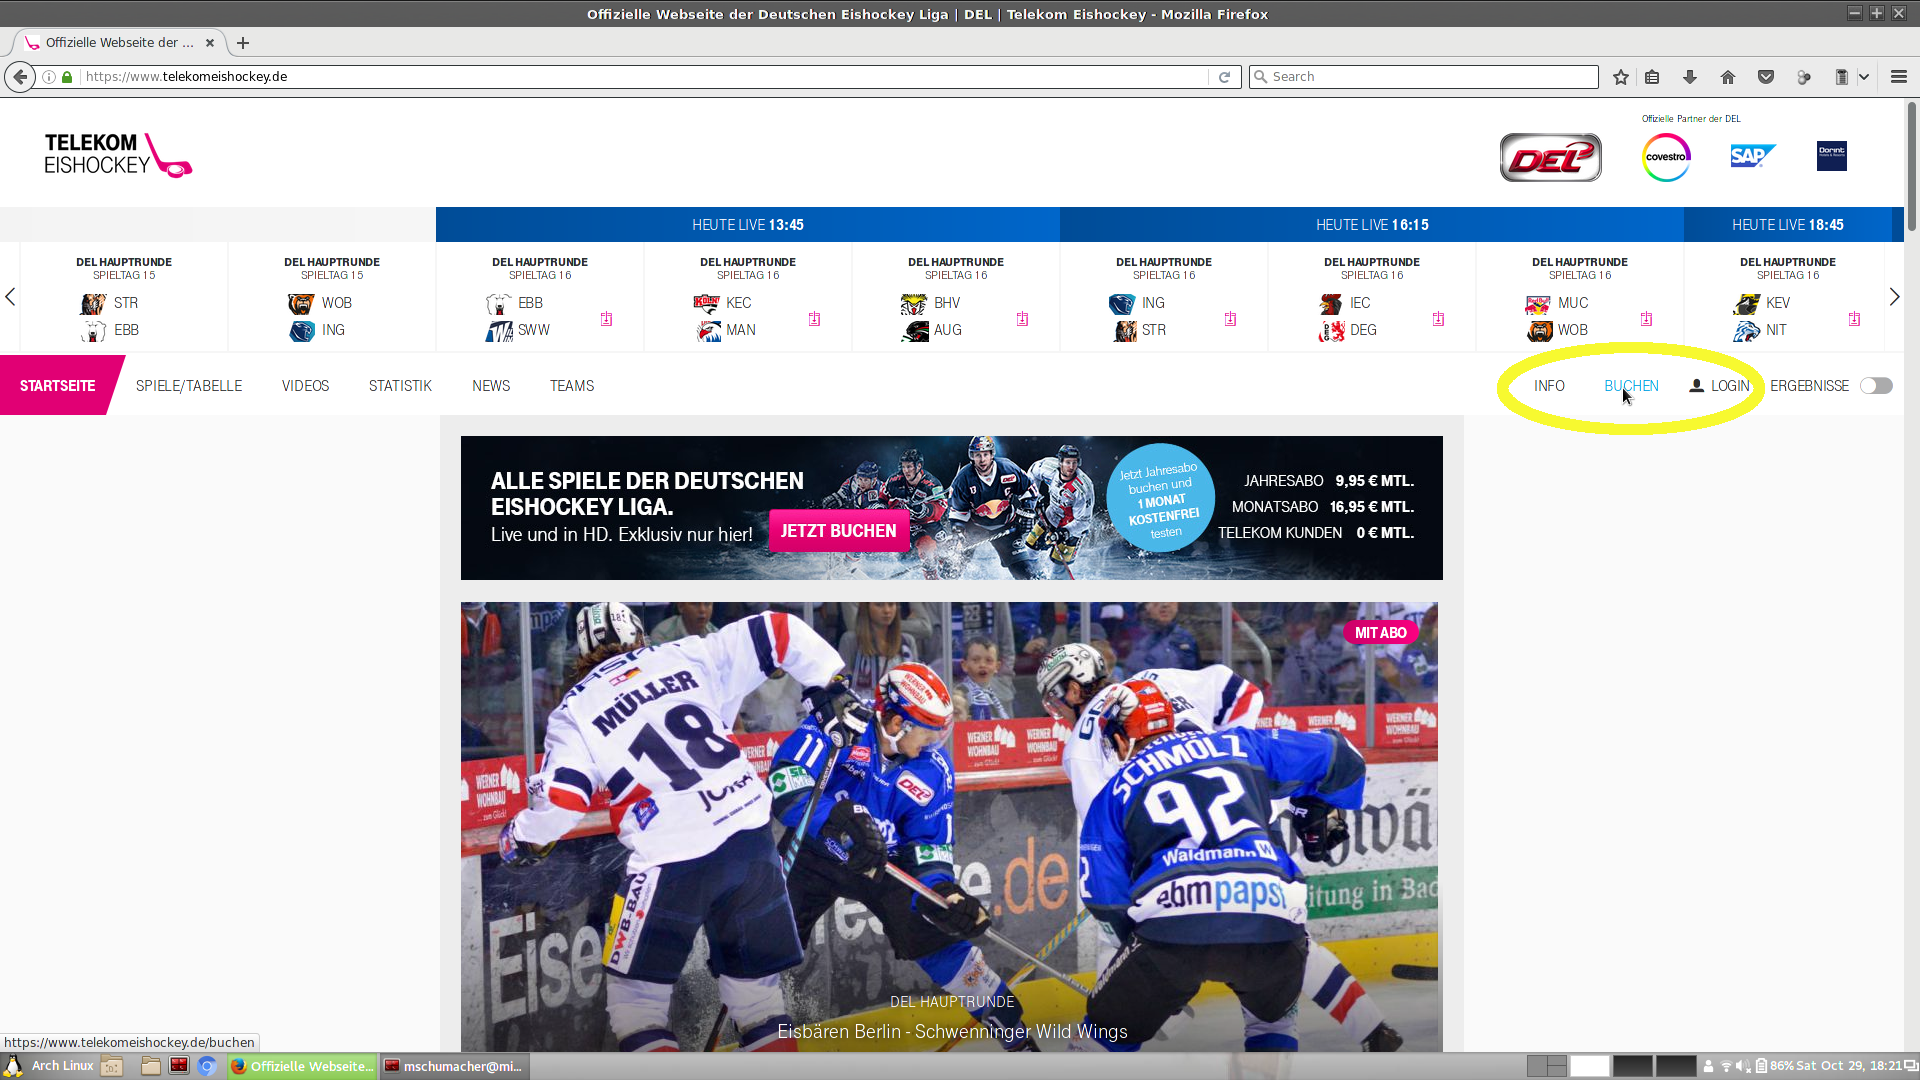
\includegraphics[width=\textwidth]{01-del_homepage.png}
		Select "BUCHEN" (book subscription) in the upper right corner.
	
	\subsection{Select subscription type}
		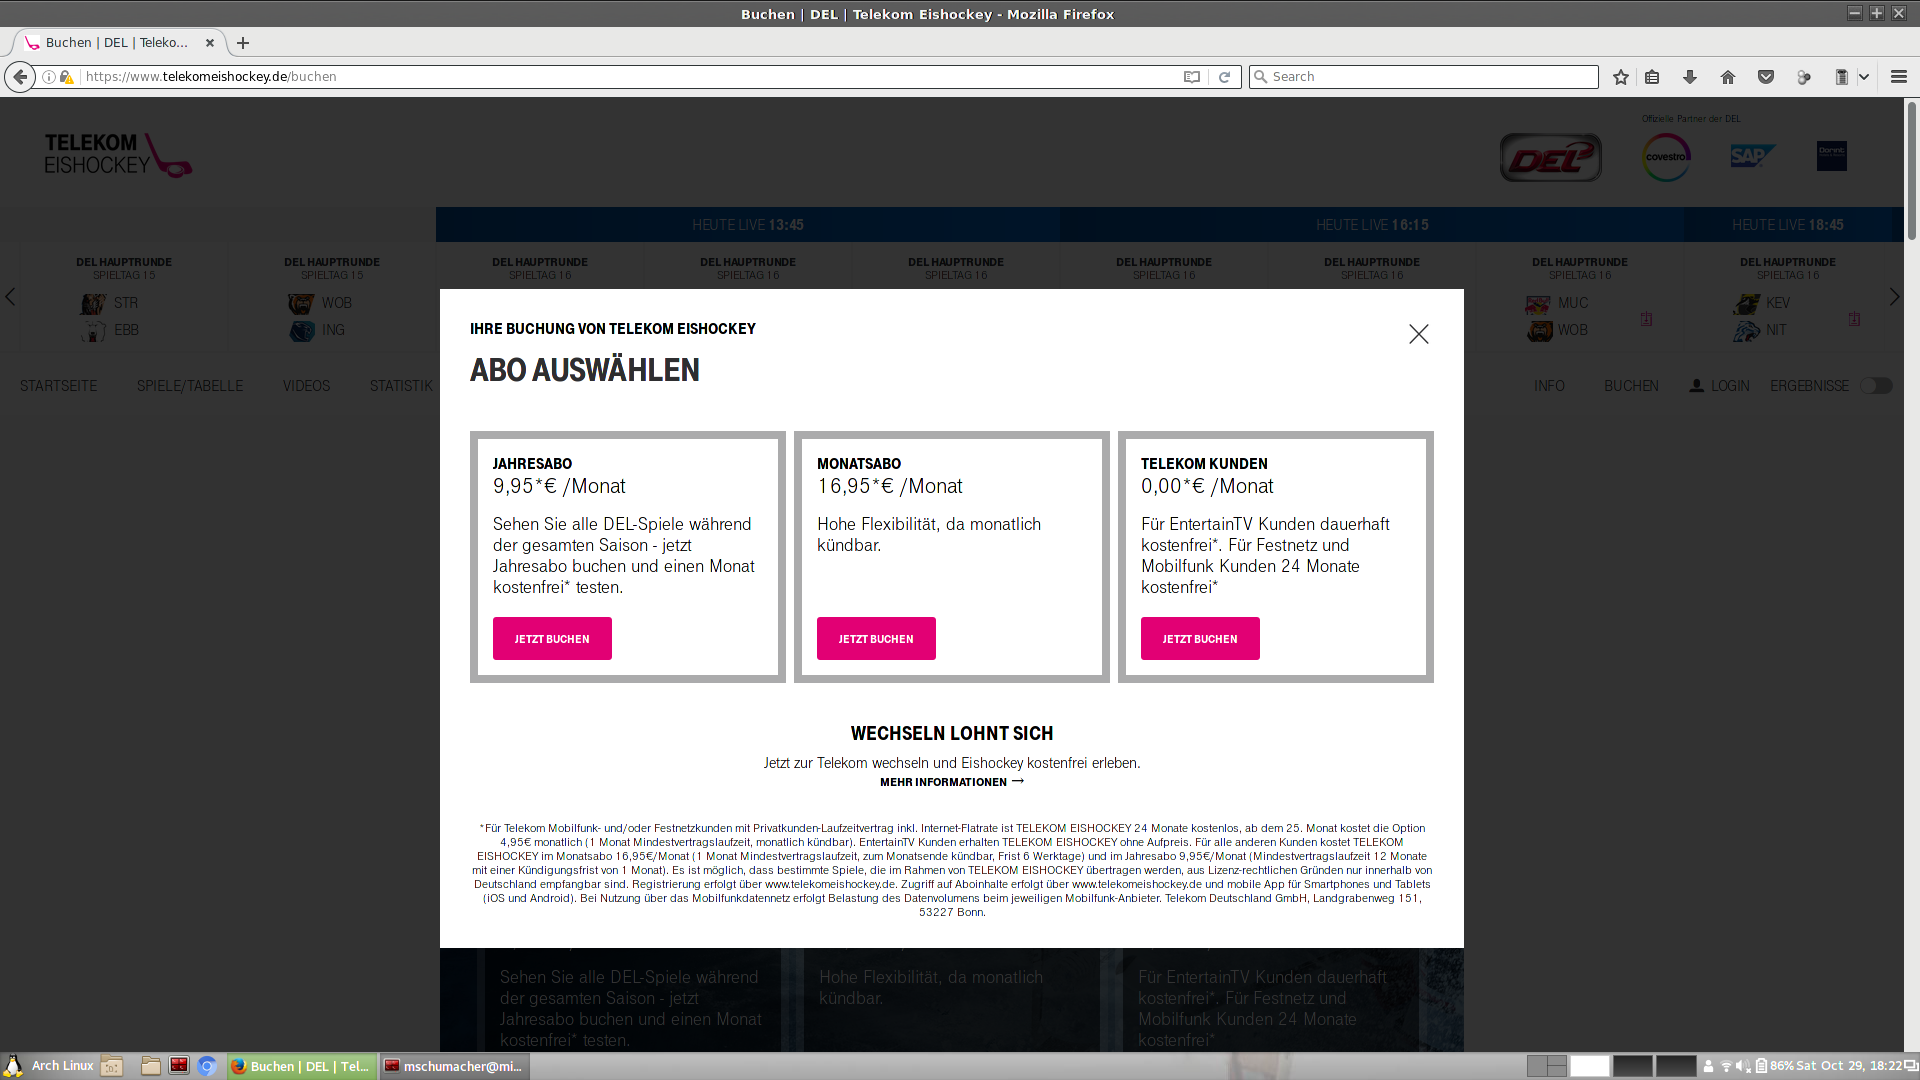
\includegraphics[width=\textwidth]{02-options.png}
		"Jahresabo" = annual subscription; "Monatsabo" = monthly subscription
		A monthly subscription would be the better deal at this point, since they play through April.
		\[ \frac{16.95}{\mbox{month}} \times 6 \mbox{ months} = 101.70 \, <  \, \frac{9.95}{\mbox{month}} \times 12 \mbox{ months} = 119.40 \]
		
	\subsection{Select to create a Telekom login}
		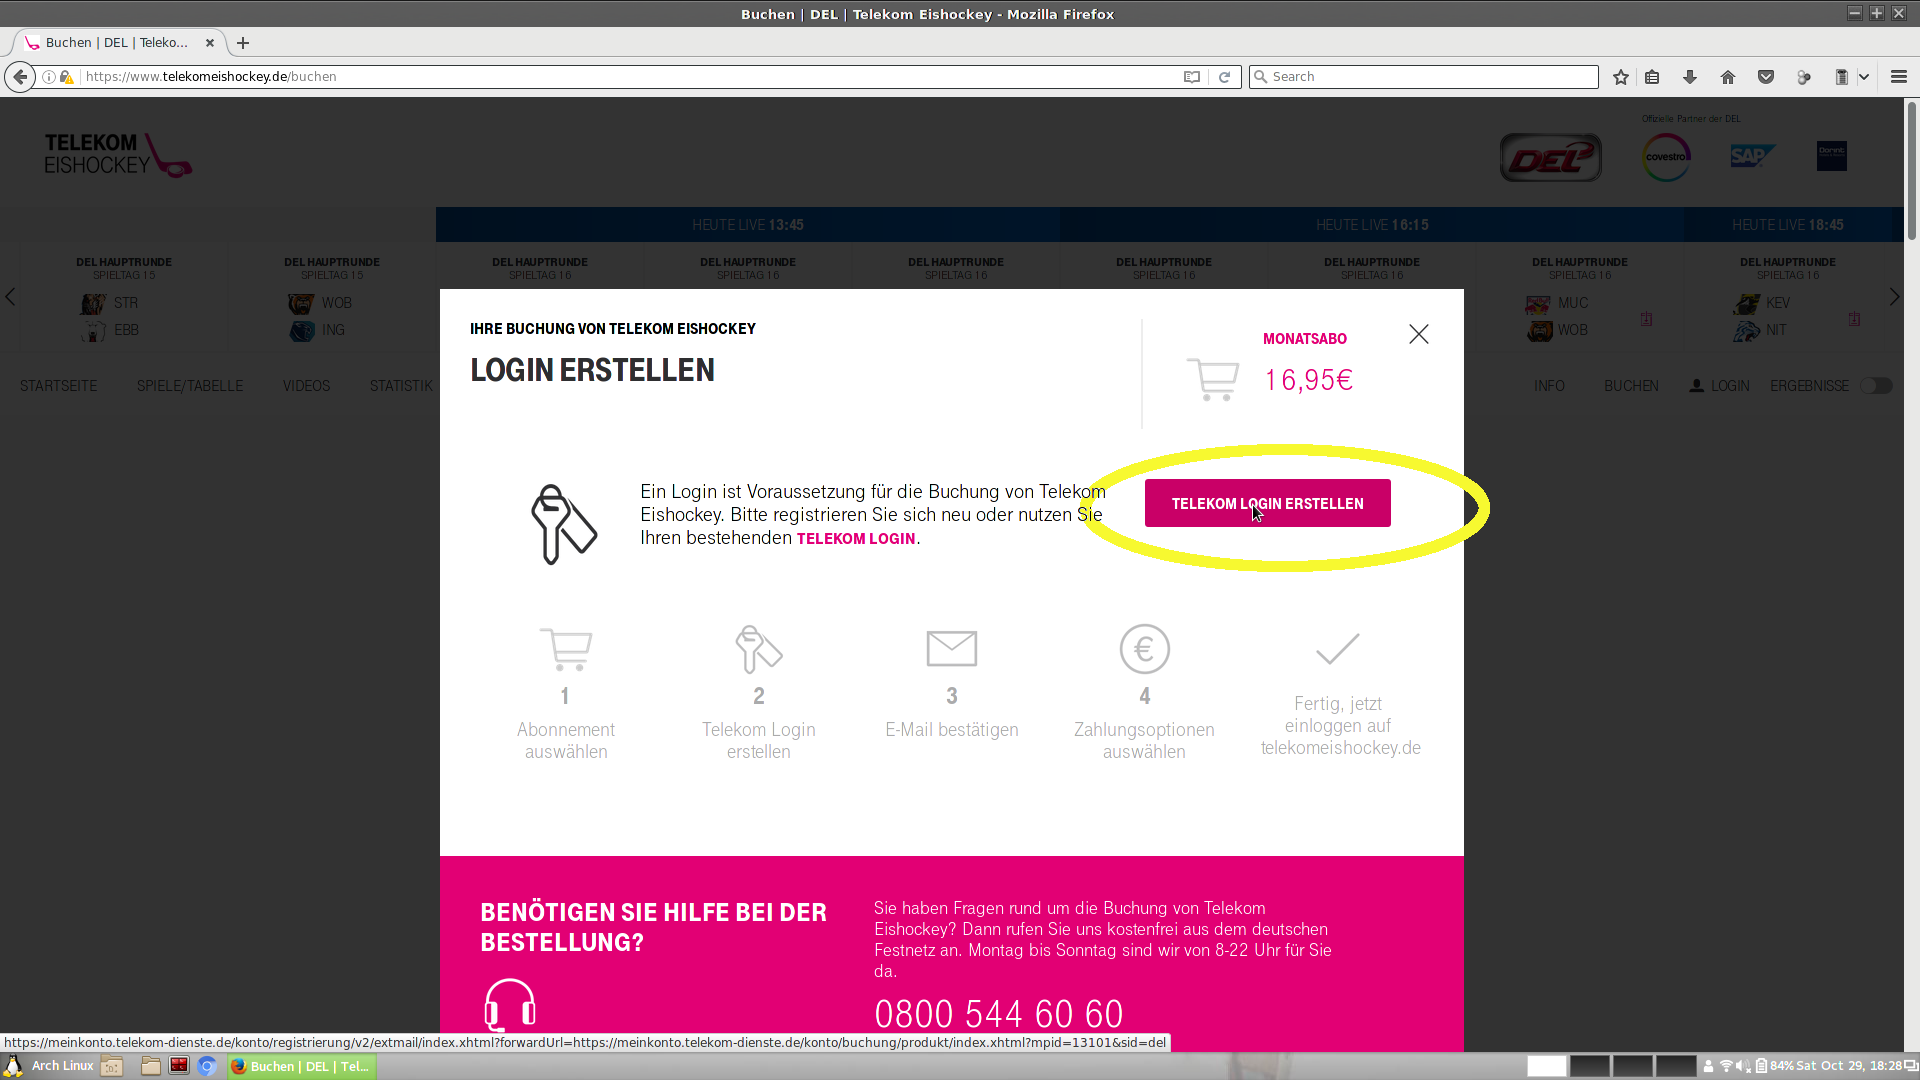
\includegraphics[width=\textwidth]{03-create_login.png}
		Click on "Telekom Login erstellen" (create Telekom login).
	
	\subsection{Enter login info}
		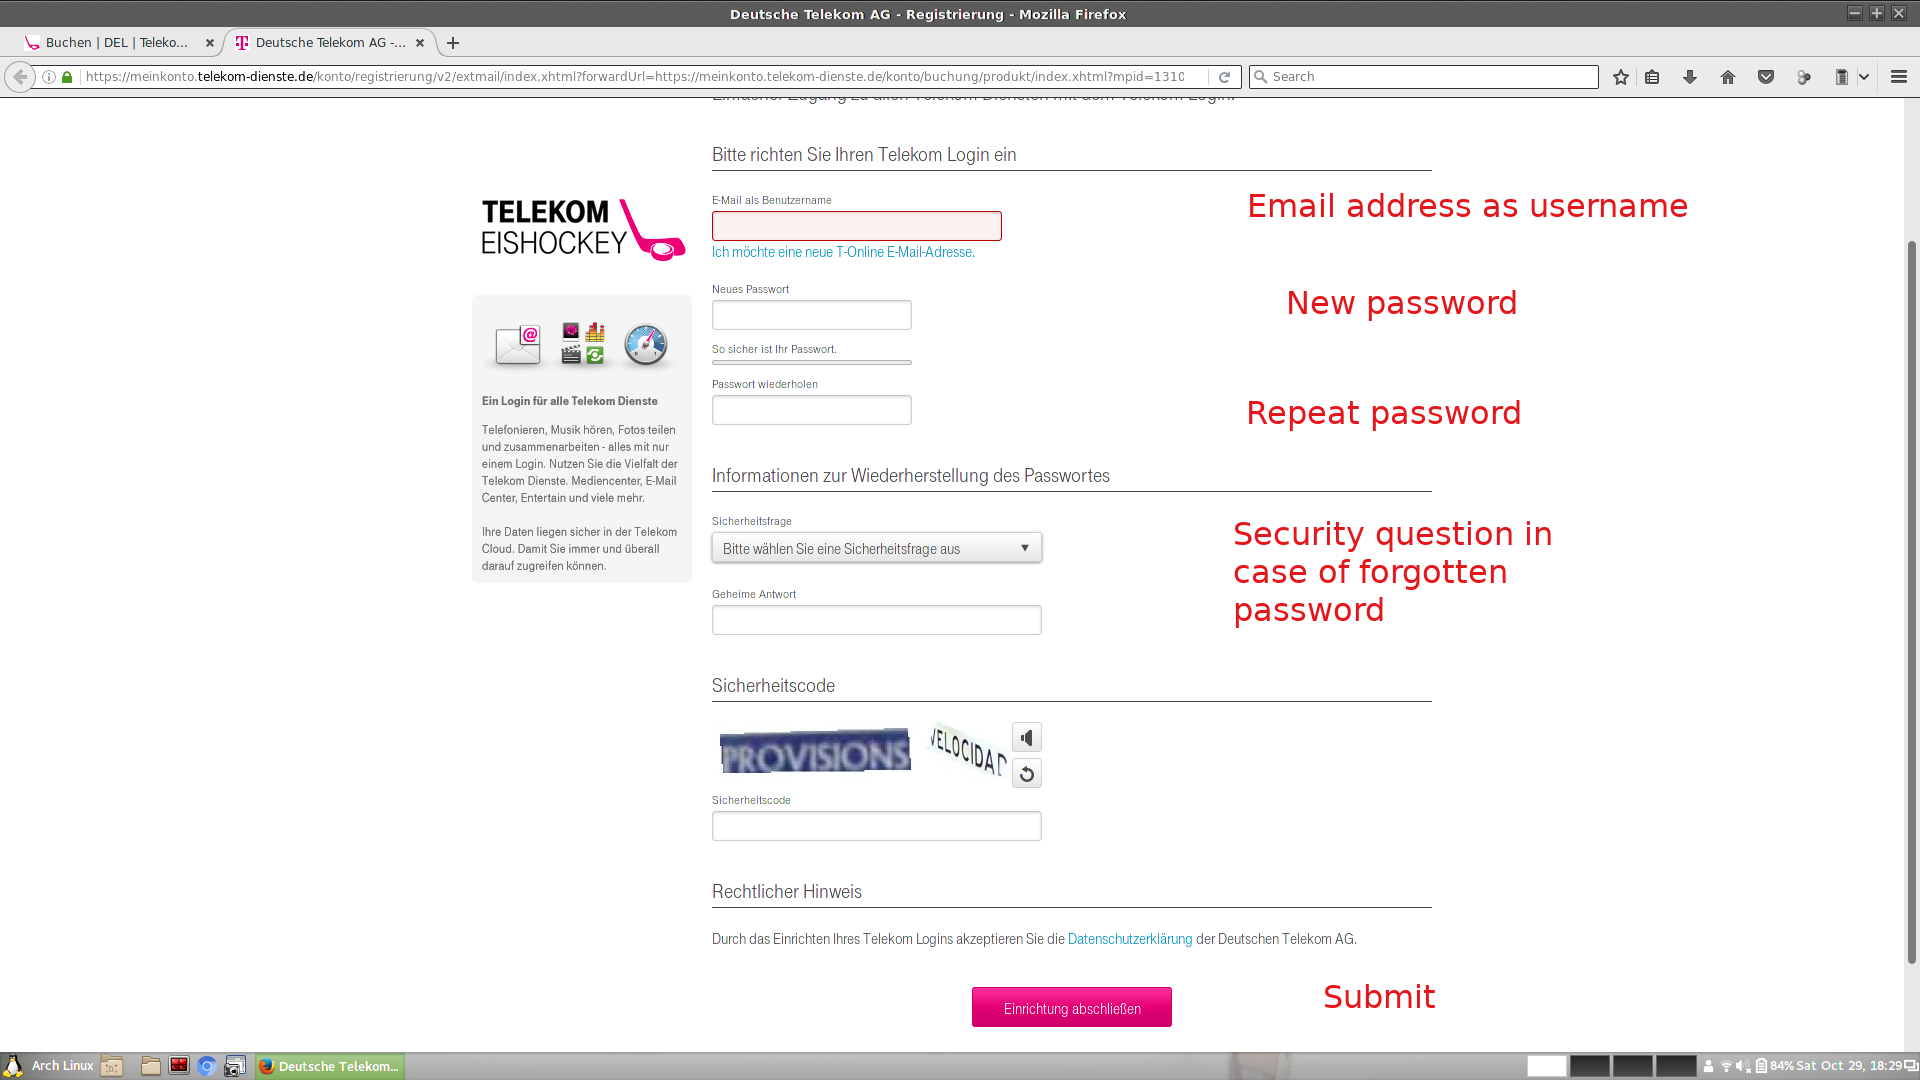
\includegraphics[width=\textwidth]{04-setup_login.png}
		\begin{flushleft}
		The security question offers the following options: \linebreak
		"Wie lautet der Beruf Ihres Grossvaters?" = grandfather's occupation \linebreak
		"Wo haben Sie Ihren Partner kennengelernt?" = where did you meet your spouse \linebreak
		"Wie lautet die Name Ihrer Grundschule?" = name of your elementary school \linebreak
		"Wie lautet Ihre Lieblingsfigur aus der Geschichte?" = favorite historical figure \linebreak
		"Was ist Ihr Lieblingshobby?" = favorite hobby \linebreak
		"Wie ist der Geburtsname Ihrer Mutter?" = mother's maiden name \linebreak
		"Welche ist Ihre Lieblingsmannschaft?" = favorite team \linebreak
		"Was war Ihr erstes Auto?" = first car \linebreak
		"Wie lautet die Vorname Ihres Vaters?" = father's first name \linebreak
		"Wie hiess der beste Freund aus Ihrer Kindheit?" = childhood best friend \linebreak
		"Wie heisst oder hiess Ihr erstes Haustier?" = name of first pet \linebreak
		"Wie ist der Name Ihres Lieblingslehrers?" = name of favorite teacher
		\end{flushleft}
		
		You will receive a verification email from "Kundencenter Deutsche Telekom" (Deutsche Telekom
		account center). Click on the link "Email-Addresse best{\"a}tigen" (confirm email address).
		
	\subsection{Select country}
		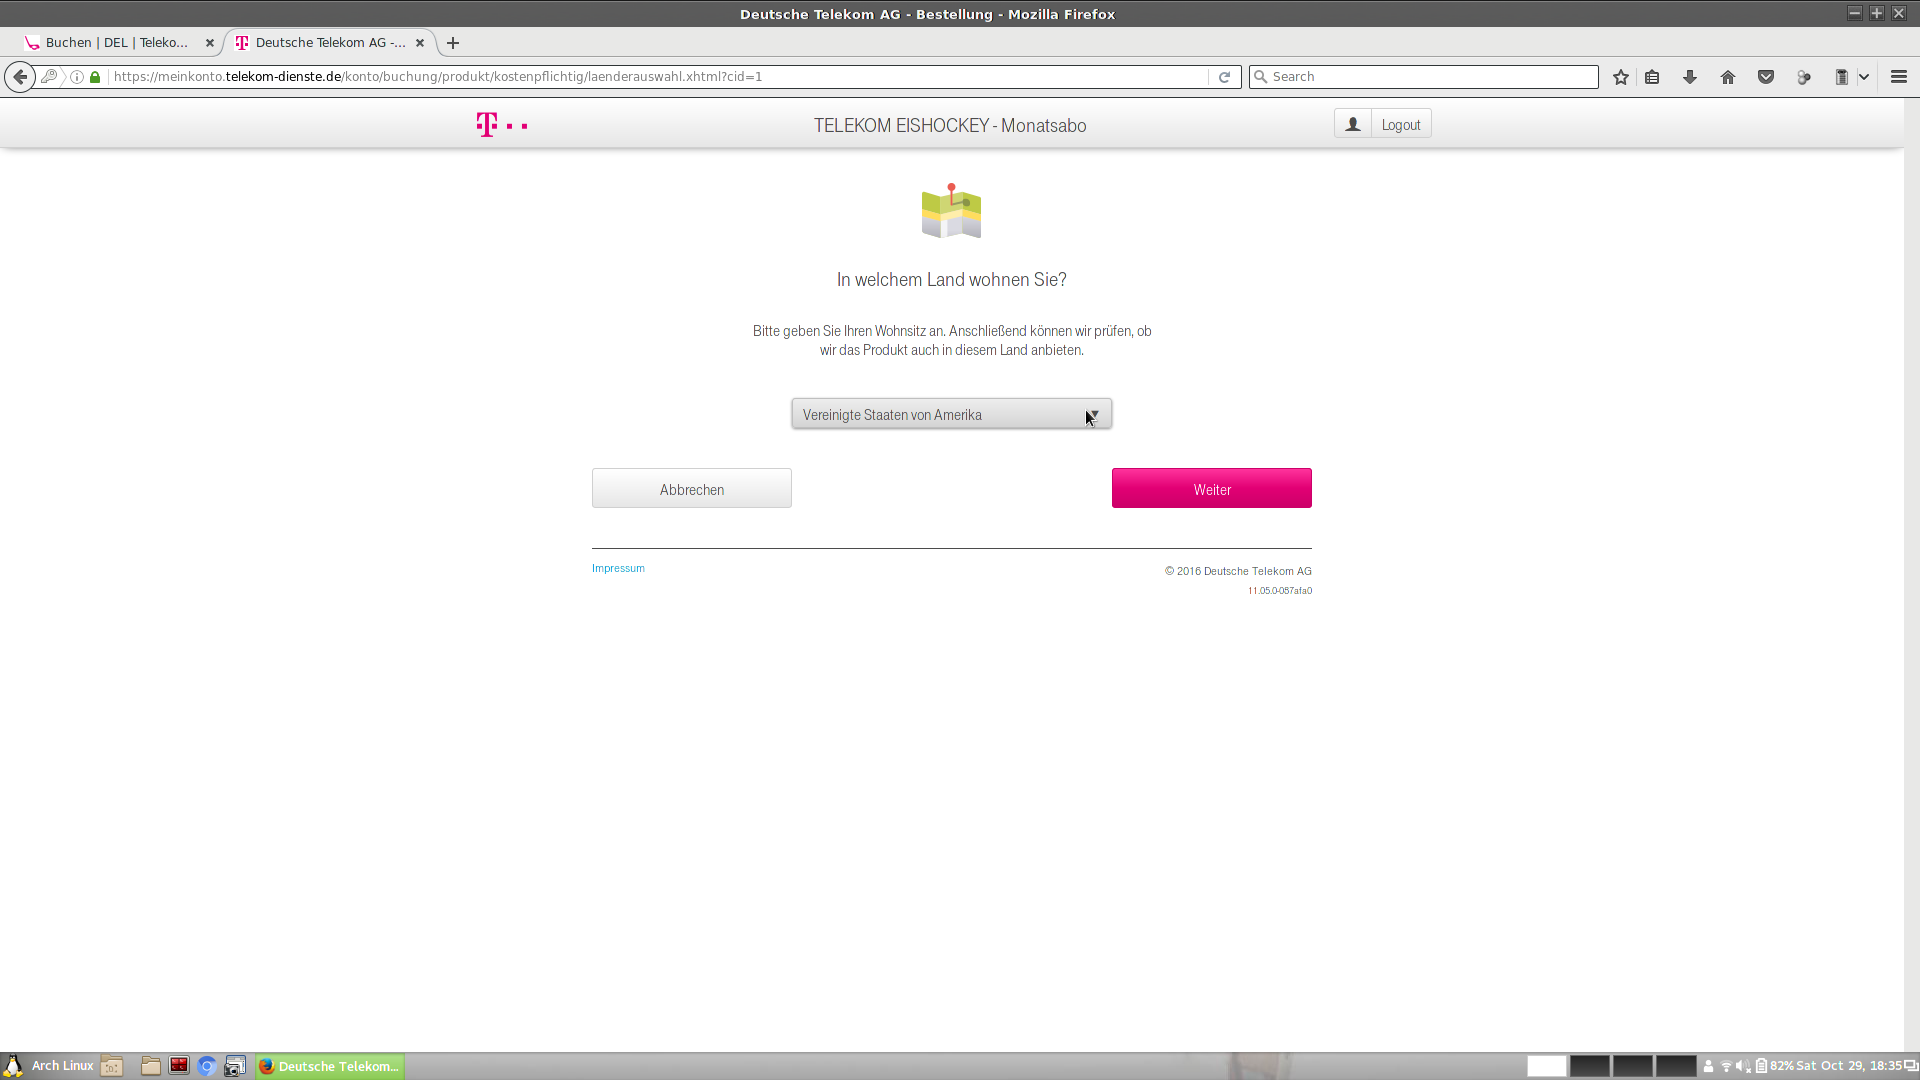
\includegraphics[width=\textwidth]{05-country.png}
		"Vereinigte Staaten von Amerika" = United States of America
	
	\subsection{Select payment method}
		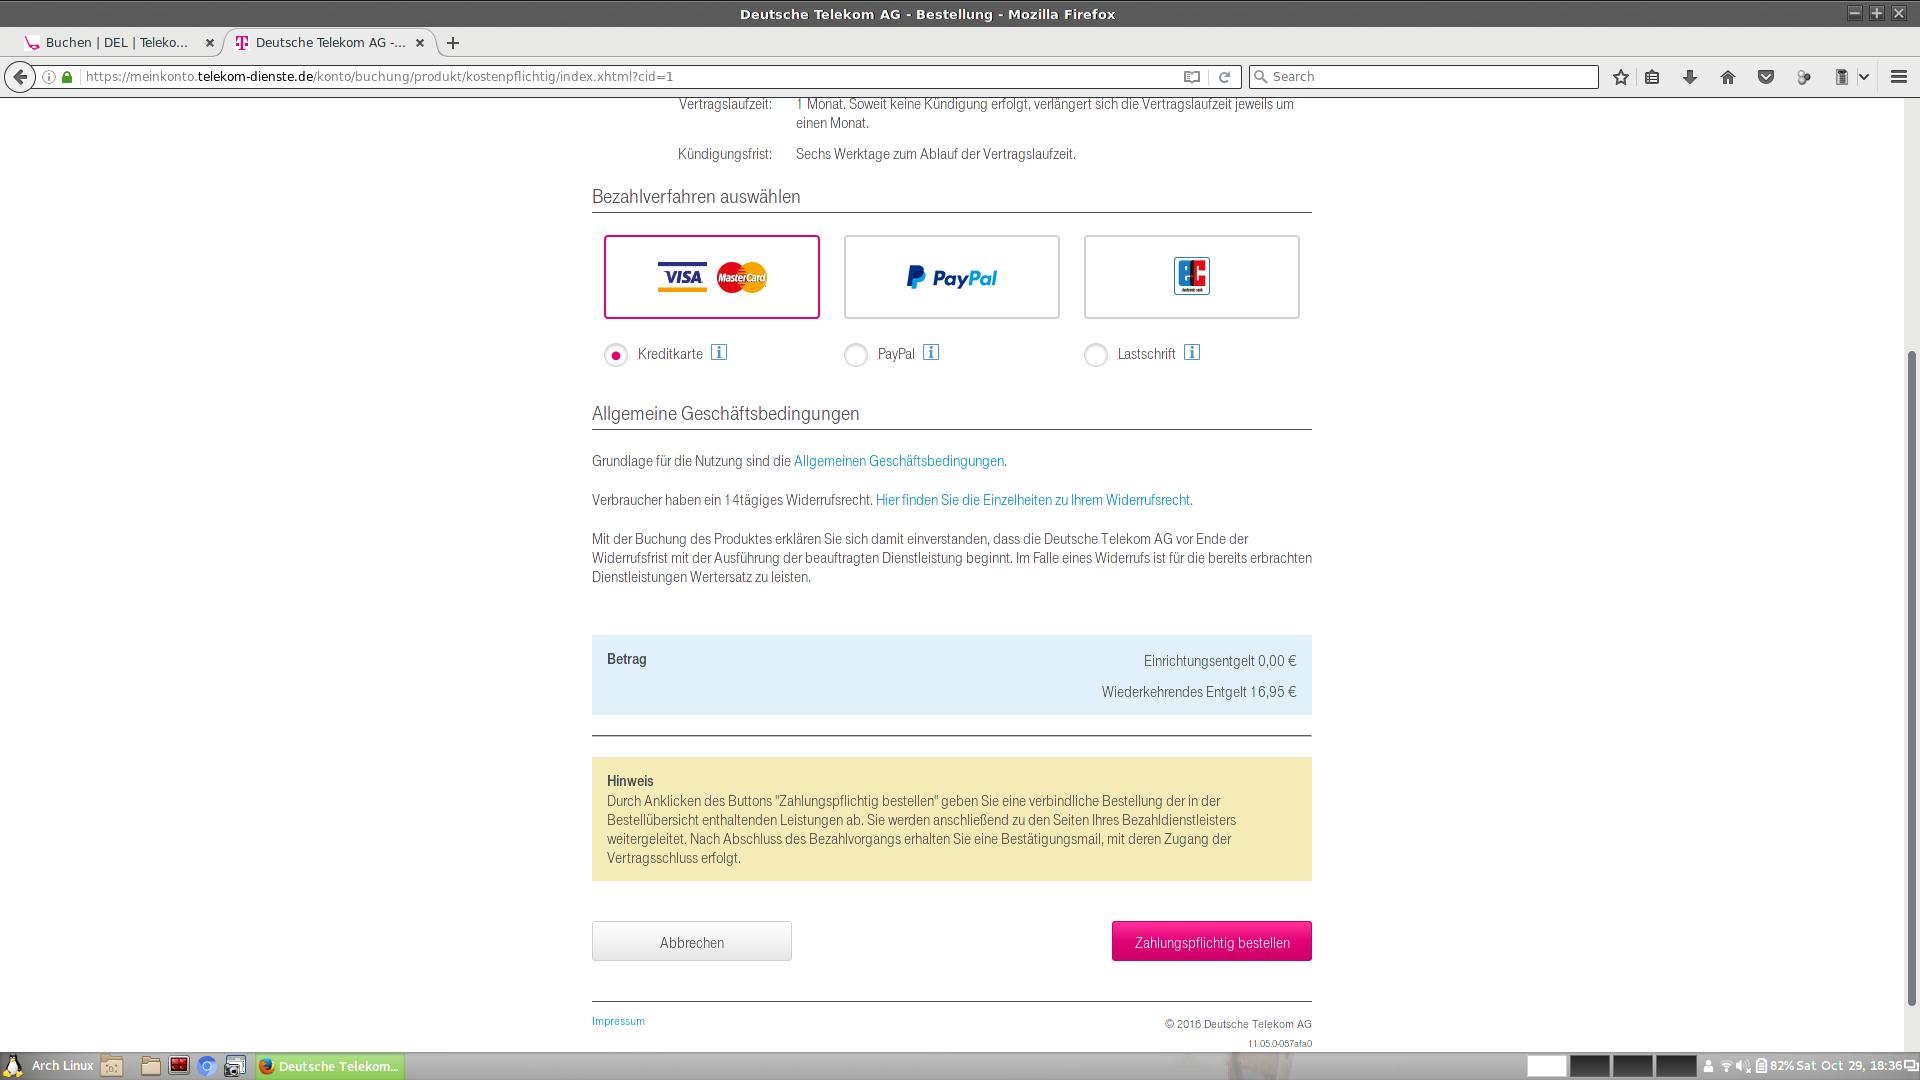
\includegraphics[width=\textwidth]{06-payment_method.png}
		"Lastschrift" is only available with European bank accounts, so your options are likely
		credit/debit or Paypal. Then click "Zahlungspflicht bestellen."
	
	\subsection{Enter card/Paypal info}
		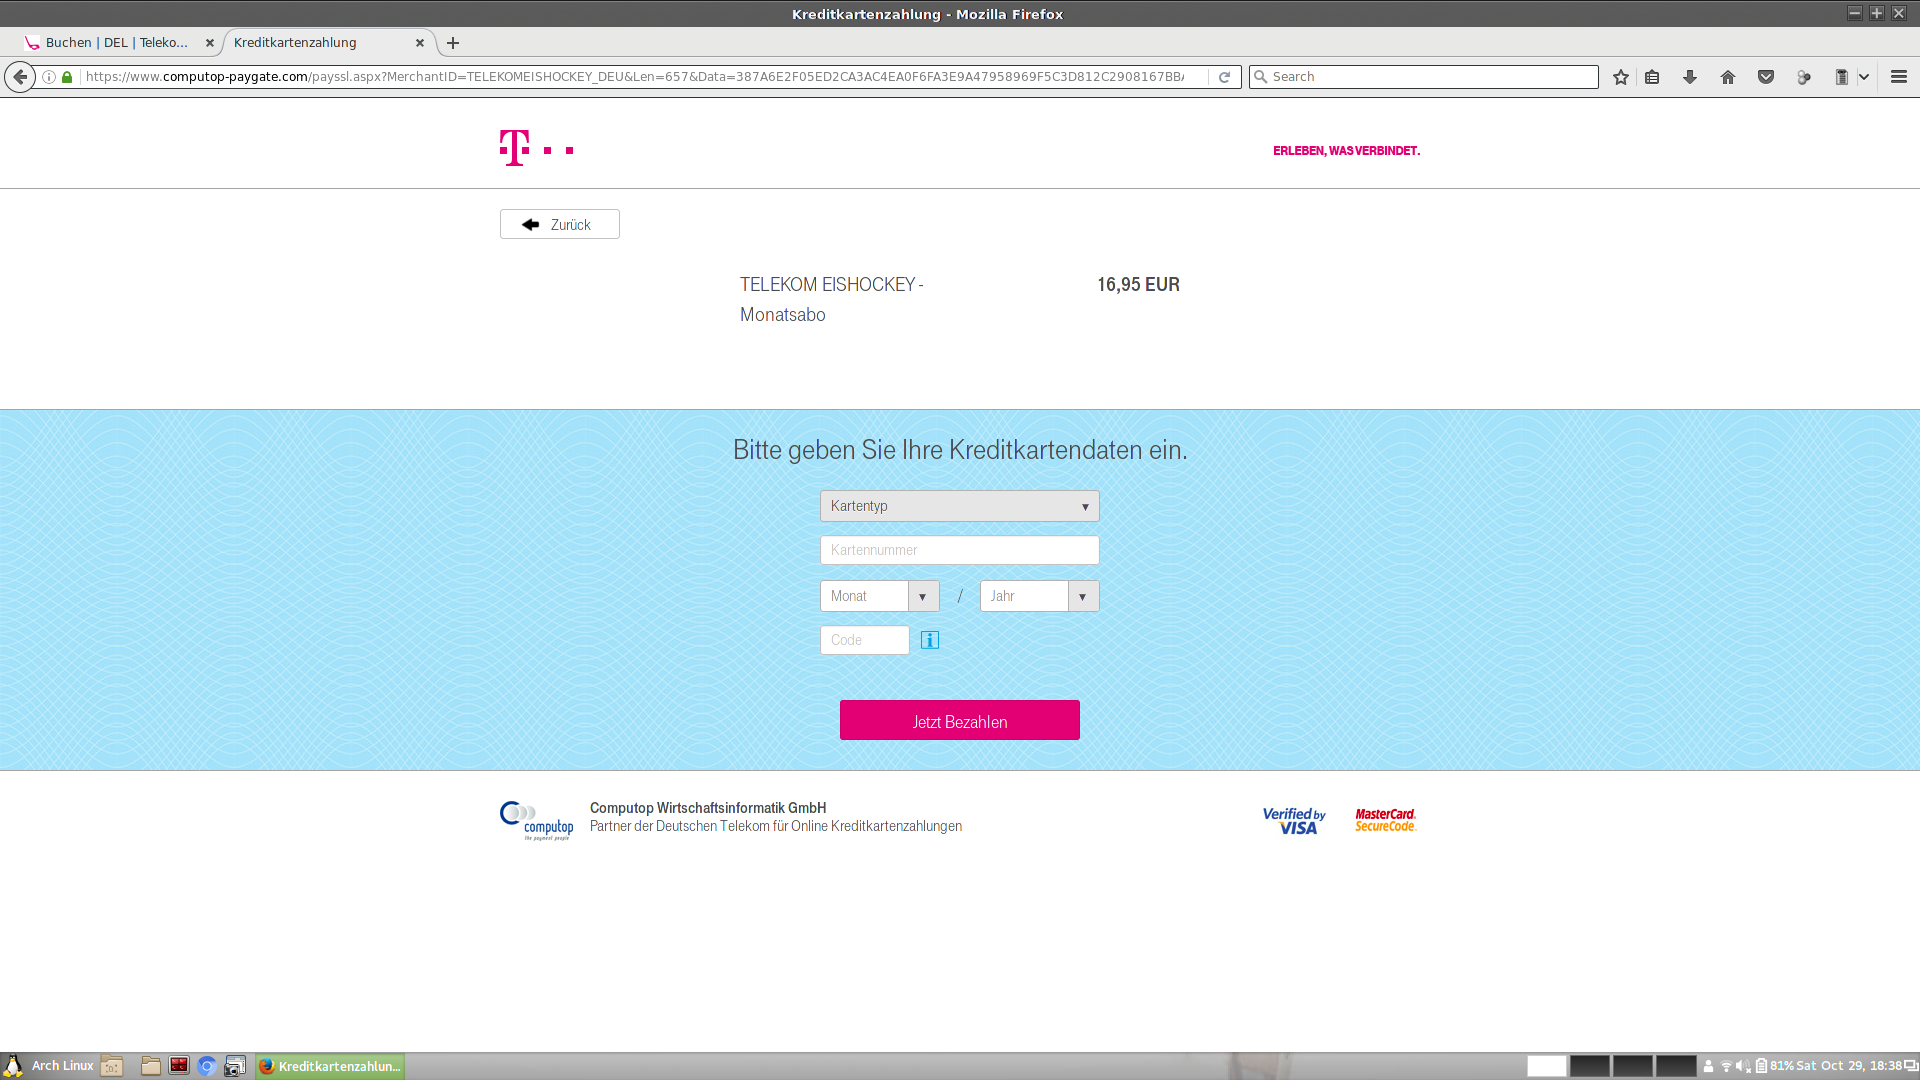
\includegraphics[width=\textwidth]{07-card_info.png}
		This page should be pretty self-explanatory. "Jetzt bezahlen" = pay now.

\section{Watch the game!}
	Just select the game. The video should start playing automatically if you are logged in and paid
	for. Past games have a highlights video, live games have the live feed. The video is FLV, and
	seems fairly platform/browser independent, so use whichever browser you prefer.
		

\end{document}